\documentclass[a4paper,10pt]{report}
\usepackage[utf8x]{inputenc}
\usepackage{amsmath}
\usepackage{amssymb}
\usepackage{graphicx}
\usepackage{glossaries}
\usepackage[menubordercolor={0 0 0}]{hyperref}
\hypersetup{menubordercolor={0 0 0}}
%opening
\title{Theoretikum}
\author{Anupam Prasad Vedurmudi}

\begin{document}

\maketitle

\begin{abstract}
 
\end{abstract}

\tableofcontents
\newpage
\section{Introduction}
In this write-up we are concerned with the theoretical analysis of scattering experiments.
The basic principle of scattering for classical particles is simple - we start with any number of particles 
(two in the simplest case) which are far apart in some sense. This means that we can assume that the particles 
don't interact with eachother in any way. After the passage of some time these particles ``collide'' or 
interact locally in some sense and after some time they are far apart again. From the initial and final 
properties (position, velocity, etc.) we can infer the details of the interaction.

In quantum scattering, however, matters are slightly more complicated. The very notion of a ``path'' with a definite velocity 
is meaningless. We instead need to calculate the probability of a particle to deviate or ``scatter'' through a given angle. This
quantity is known as the differential cross-section. Although it is the fundamental quantity of interest in scattering theory,
our focus in this write-up will be on a tool that is indirectly related to it - the Born series. We note that quantum scattering
theory can be further divided into nonrelativistic and relativistic cases. In this write-up we are only concerned with the former case.

The Born series is a perturbation expansion that enables us to calculate the Scattering operator to a desired order. 
The Scattering operator calculates the final state given a specific initial state. This can then be used to compute the
cross-section. The objects of interest that can be studied using this method are the Green's function and the T operator.
\section{Preliminaries}

This section is based on the textbook, \cite{TaylorScattering}
and the first part of the lecture notes, \cite{YafaevScattering}. The problem is of the scattering of a single particle off
a potential. It can be shown that this problem is equivalent to that of two-particle
scattering.
We define the Hamiltonian operator as,
\begin{equation}
 H = H_0+V\\
\end{equation}
 Where, $H_0$ is the free Hamiltonian given by, 
\begin{equation}
 H_0=-\frac{\Delta}{2}
\end{equation}
 $\Delta$ is the Laplace operator and $V$ corresponds to the potential. 
For convenience, we work in units where, $\hbar^2/m=1$. Here, $m$ is the
mass of the particle.

\subsection{Spectrum of The Hamiltonian}
 $H_0$ and $H$ are self-adjoint operators on a Hilbert space
$\mathcal{H}$. In general, the spectrum of a self-adjoint operator has
two components,
\begin{itemize}
 \item Discrete - corresponding to the bound states
 \item Continuous - corresponding to the scattering states
\end{itemize}
The continuous part of the spectrum can be further divided into into
an $absolutely$ $continuous$ and a $singular\ continuous$ part. This results in a
corresponding decomposition of the Hilbert space into three invariant subspaces.
\begin{equation}\label{HilbertDecomp}
 \mathcal{H}=\mathcal{H}^{pp}\oplus\mathcal{H}^{ac}\oplus\mathcal{H}^{sc}
\end{equation}
 Where, $\mathcal{H}^{pp}$ is the part of the Hilbert space corresponding to
the discrete (pure point) part of the spectrum. For most systems of interest, the singular continous 
part is absent. Scattering theory is essentially perturbation theory applied on the 
absolutely continous part of the spectrum.

The spectrum of $H_0$ only contains an absolutely continuous part - the positive real axis including $0$. We denote the eigenstates of
$H_0$ as $|\mathbf{k}\rangle$, where $\mathbf{k}\in\mathbb{R}^3$. The eigenvalue corresponding to these eigenstates is $E=k^2/2$,
$k=|\mathbf{k}|$. These eigenstates are improper, i.e., they are not normalisable,
\begin{equation}\label{FreeNormalisation}
 \langle\mathbf{k}^{\prime}|\mathbf{k}\rangle=\delta\left(\mathbf{k}^{\prime}-\mathbf{k}\right)
\end{equation}
Where $\delta$ is the Dirac delta function. The reason for the notation is that, the wavefunction corresponding this eigenstate is given by,
\begin{equation}\label{FreeWavefunction}
  \langle\mathbf{x}|\mathbf{k}\rangle = e^{i\mathbf{k}.\mathbf{x}}
\end{equation}
The eigenstates corresponding to the discrete part of the spectrum are called the \emph{bound} states and those of the continuous
part are called the \emph{scattering} states. We will later see that the scattering states asymptotically look like free-eigenstates while
the bound states don't.
\vspace{\baselineskip}

\subsection{Time Evolution and The Asymptotic Condition}
 In the Schrödinger picture, the time evolution of a state $|\psi_t\rangle$ is given by,
\begin{equation}\label{SchroedingerEvolution1}
 i\frac{d}{dt}|\psi_t\rangle = H|\psi_t\rangle
\end{equation}
Given an initial state $|\psi\rangle$, the formal solution of \eqref{SchroedingerEvolution1}
given by,
\begin{equation}\label{TimeEvolution}
 |\psi_t\rangle = U(t)|\psi\rangle 
\end{equation}
Where, $U(t)=e^{-iHt}$. Since $H$ is self-adjoint, $U(t)$ is a unitary operator on $\mathcal{H}$, i.e., it is a linear operator that
maps the whole of the Hilbert space onto itself and preserves the norm. Put more precisely, 
\begin{equation*}
\mathcal{D}\left(U(t)\right)=\mathcal{R}\left(U(t)\right)=\mathcal{H}
\end{equation*}
And, $\Arrowvert\Omega\psi\Arrowvert=\Arrowvert\psi\Arrowvert$. As a consequence, we are led a useful property of unitary operators, 
\begin{equation}\label{unitaryprop}
  U^\dagger(t)U(t)=U(t)U^\dagger(t)=\mathbb{I}
\end{equation}

The essence of scattering theory is that \eqref{TimeEvolution} describes the evolution of some scattering wavefunction such that,
\begin{align}\label{Asymptotic1}
 U(t)|\psi\rangle &\displaystyle\xrightarrow[t\rightarrow-\infty]{}  U^0(t)|\psi_{in}\rangle\\
 U(t)|\psi\rangle &\displaystyle\xrightarrow[t\rightarrow+\infty]{}  U^0(t)|\psi_{out}\rangle
\end{align}
Where, $U^0(t)=e^{-iH_0t}$ is the free evolution operator and $|\psi_{in}\rangle$ and $|\psi_{out}\rangle$ are the in and out
states. The in and out states behave like free wave-packets - i.e., their time evolution is governed by the free Hamiltonian.

The asymptotic condition states that for every $|\psi_{in}\rangle$ in $\mathcal{H}$ there is a $|\psi\rangle$ such that 
\eqref{Asymptotic1}.

\subsection{Green's Operator}
The Green's operator is formally defined as,
\begin{align}\label{GFdefinition}
 G\left(E\pm i0\right) &=\left(E\pm i0-H\right)^{-1}\\
 G_0\left(E\pm i0\right) &=\left(E\pm i0-H_0\right)^{-1}
\end{align}
Where, $G\left(E\pm i0\right)=\displaystyle\lim_{\epsilon\rightarrow 0}G(E\pm i\epsilon)$. The
Lippmann-Schwinger equation for the Green's operator is given by,
\begin{equation}\label{LS1}
 G=G_0+G_0VG
\end{equation}
 The above equation can be derived by using the matrix identity,
\begin{equation}\label{MatrixIdentity1}
	A^{-1}=B^{-1}+A^{-1}\left(B-A\right)B^{-1}
\end{equation}

Subsequently, an operator-series expansion for $G$ is obtained by iteratively substituting
the $(n-1)^{th}$ order approximation for $G$ in the R.H.S of \eqref{LS1} to get the $n^{th}$
order term. The $0^{th}$ order approximation is the free Green's operator $G_0$, the $1^{st}$
order approximation (the Born approximation) is given by,

\begin{equation}\label{BornApproximation}
 G=G_0+G_0VG_0
\end{equation}
The Born series for the Green's operator can thus be written as,
\begin{equation}\label{BornSeriesExpanded}
 G=G_0+G_0VG_0+G_0VG_0VG_0+\ldots
\end{equation}
Or more compactly,
\begin{equation}\label{BornSeriesCompact}
 G=\displaystyle\sum_{n=0}^{\infty}G_0\left(VG_0\right)^n
\end{equation}

\subsection{T-Operator}
As described in \cite{TaylorScattering}, it is convenient to define the $T$-operator,
\begin{equation}\label{Toperator1}
 T=V+VGV
\end{equation}
 Multiplying both sides by $G_0$ we get and using \eqref{LS1}, we get,
\begin{equation}\label{TOperatorRelation1}
 G_0T=GV
\end{equation}
 Substituting this relation back in \eqref{Toperator1} we get a Lippmann-Schwinger equation
for the $T$-Operator,
\begin{equation}\label{LS2}
 T=V+VG_0T
\end{equation}
 And correspondingly, through iteration, a Born Series,
\begin{equation}\label{BornSeriesToperator}
 T=\displaystyle\sum_{n=0}^{\infty}V\left(G_0V\right)^n
\end{equation}
The Born approximation in this case is, $T\simeq V$.

The momentum space matrix elements of the T-matrix are given by,
\begin{equation}\label{Tmatrixelements}
  t\left(\mathbf{k}^\prime\leftarrow\mathbf{k}\right)=\langle \mathbf{k}^\prime |T| \mathbf{k} \rangle
\end{equation}

\subsection{Scattering Operator}
We first define the Møller operators, $\Omega_\pm$ as,
\begin{equation}\label{moellerdef}
 \Omega_\pm = \displaystyle\lim_{t\rightarrow\mp\infty}U(t)^\dagger U^0(t)
\end{equation}
These operators act on the in and out states to give,
\begin{align}\label{moelleract}
 |\psi\rangle &=\Omega_+|\psi_{in}\rangle \\
 |\psi\rangle &=\Omega_-|\psi_{out}\rangle 
\end{align}

The Møller wave operators acting on an in or out state give the corresponding scattering state
for the Hamiltonian. These operators are isometric, i.e., they are defined on all of $\mathcal{H}$
and preserve the norm. They differ from unitary operators in that, $\mathcal{R}\left(\Omega_\pm\right)\neq\mathcal{H}$.
Unlike the property \eqref{unitaryprop} for unitary operators, we have $\Omega_\pm^\dagger\Omega_\pm=\mathbb{I}$, but
in general, $\Omega_\pm\Omega^\dagger_\pm\neq\mathbb{I}$. We also note that all Unitary operators are isometric.We 
can now define the scattering operator,
\begin{equation}\label{scatteringopdef}
 S=\Omega_-^\dagger\Omega_+
\end{equation}
The scattering operator has the property that,
\begin{equation}\label{scatterinprop}
 |\psi_{out}\rangle = S|\psi_{in}\rangle
\end{equation}
i.e., given an in state, the scattering operator gives the corresponding out state. In practice, only the asymptotic free motion 
is observable. Therefore, the operator $S$ contains all the information of experimental interest. For a scattering process,
$|\psi_{in}\rangle\rightarrow|\psi_{out}\rangle$, the probability is given by,
\begin{equation}\label{scatteringprob}
 \mathbf{w}(|\psi_{out}\rangle\leftarrow|\psi_{in}\rangle)=\lvert\langle\psi_{out}\rvert S\lvert\psi_{in}\rangle\rvert^2
\end{equation}

The momentum space matrix elements of the scattering operator are related to \eqref{Tmatrixelements} as,
\begin{equation}\label{Smatrixelements}
 \langle \mathbf{k}^\prime |S| \mathbf{k} \rangle = \delta_3(\mathbf{k}^\prime - \mathbf{k})-2\pi i\delta\left(E_{p^\prime}-E_p\right)t\left(\mathbf{k}^\prime\leftarrow\mathbf{k}\right)
\end{equation}

\section{Finite Element Method}
The Finite Element Method (FEM) is a numerical technique used to solve differential equations.
The method exploits the locality of the differential operator. The solution space is divided into
subspaces. These subspaces take the form of a mesh, i.e., a collection of simplices - triangles
in 2D, tetrahedra in 3D, etc. The function is then approximated using smooth basis functions with support in these subspaces.
These basis functions with finite support are referred to as finite elements.

Let $\psi$ be a solution to a differential equation. We denote the basis functions by $\phi_n$,
\begin{equation}\label{femfirst}
 \psi(\mathbf{x})\simeq\widetilde{\psi}(\mathbf{x})=\displaystyle\sum_n^N c_n\phi_n(\mathbf{x})
\end{equation}

A feature of FEM is that the basis functions have a finite overlap i.e., they are not orthogonal.
The overlap matrix in general has a block-diagonal form. The overlap matrix is denoted by,
\begin{equation}\label{overlap}
 S_{nm}=\int d^3x\phi_n(\mathbf{x})\phi_m(\mathbf{x})
\end{equation}

We also define the matrix,
\begin{equation}\label{diff_overlap}
 B_{nm}=\int d^3x\nabla\phi_n(\mathbf{x}).\nabla\phi_m(\mathbf{x})
\end{equation}

\subsection{Boundary Conditions}
In order to solve the differential equations we must also specify appropriate boundary
conditions. Let $\Omega$ be the solution space. We denote its boundary by $\partial\Omega$.

\subsubsection{Dirichlet Boundary Condition}
The Dirichlet boundary condition requires that the function has a known value on the boundary.
\begin{equation}\label{dirichlet1}
 \psi(\mathbf{x})=f(\mathbf{x}), \mbox{ }\forall\mathbf{x}\in \partial\Omega
\end{equation}
Where, $f$ is a known function on $\Omega$.

\subsubsection{Neumann Boundary Condition}
The Neumann boundary condition requires that the gradient of the function
normal to the boundary is fixed to a known function. That is,
\begin{equation}\label{neumann1}
 \frac{\partial\psi(\mathbf{x})}{\partial\mathbf{n}}\equiv\nabla\psi(\mathbf{x}).\mathbf{n} = f(\mathbf{x}), \mbox{ }\forall\mathbf{x}\in \partial\Omega
\end{equation}

\subsubsection{Mixed Boundary Condition}
It is also possible to have a boundary such that the function has a Dirichlet boundary
condition on one part (denoted by $\partial\Omega_D$) and a Neumann boundary condition
on the other ($\partial\Omega_N$).

\subsection{Python Implementation}
\section{FEM in Quantum Mechanics}
The Schrödinger equation for a wave function $\psi$ is given by,

\begin{equation}\label{schroedinger1}
 -\frac{\Delta}{2}\psi+V(\mathbf{x})\psi=E\psi
\end{equation}

 Using the FEM approximation defined in \eqref{femfirst},
\begin{equation}\label{schroedinger}
 -\frac{\Delta}{2}\displaystyle\sum_n^N c_n\phi_n(\mathbf{x})+\displaystyle\sum_n^N c_n V(\mathbf{x})\phi_n(\mathbf{x})=E\displaystyle\sum_n^N c_n\phi_n(\mathbf{x})
\end{equation}
 We get the weak formulation of the problem by multiplying both sides by $\phi_m(\mathbf{x})$ and integrating over. After integrating by parts, the kinetic term gives us
the following matrix element,
\begin{equation}\label{kineticterm}
 \int d^3x\phi_m(\mathbf{x})\Delta\phi_n(\mathbf{x}) = -\int d^3x\nabla\phi_m(\mathbf{x}).\nabla\phi_n(\mathbf{x}) = -B_{mn}
\end{equation}

 The potential term is calculated from the known functions $\phi_n$ and is defined as,
\begin{equation}\label{potentialterm}
 \int d^3xV(\mathbf{x})\phi_m(\mathbf{x})\phi_n(\mathbf{x}) = V_{mn}
\end{equation}

 Finally, the R.H.S is given by,
\begin{equation}
 E\int d^3x\phi_m(\mathbf{x})\phi_n(\mathbf{x})=ES_{mn}
\end{equation}

 We define the coefficient vector $\mathbf{\underline{c}}=[c_1,c_2,\ldots,c_N]^T$. The Schrödinger equation reduces to 
the following eigenvalue problem,
\begin{equation}\label{schroedingerfem}
  H\mathbf{\underline{c}}=ES\mathbf{\underline{c}}
\end{equation}
 Where, $H=\left(\frac{B}{2}+V\right)$

The inner product of two wavefunctions $\phi$ and $\chi$ is given by,
\begin{align}\label{innerproduct}
 \int d^3x \chi^*(\mathbf{x})\psi(\mathbf{x}) &=& \displaystyle\sum_{m,n}^{N}c_md_n\int d^3x \phi_m(\mathbf{x})\phi_n(\mathbf{x})\\
 &=& \mathbf{c}^{\dagger}S\mathbf{d}
\end{align}
 Where, $\mathbf{c}^{\dagger}=(\mathbf{c}^*)^T$.

\subsection{Momentum Eigenstates}
We now want to find an FEM representation for free eigenstate of momentum $\mathbf{k}$ (energy,
$E_k=|\mathbf{k}|^2/2$). 
It is most convenient to do so by defining a ``cosine eigenvector'',
\begin{equation}\label{cosevec}
 |\mathbf{k}\rangle = exp(-i\mathbf{k}.\mathbf{x}) + exp(i\mathbf{k}.\mathbf{x})
\end{equation}
These can be obtained by ``solving'' the free Schrödinger equation on a grid with open
boundaries, i.e., by solving the eigenvalue problem,

\begin{equation}\label{freeschroedinger}
 H_0\psi=\lambda S\psi
\end{equation}
for $\psi$.

$|\mathbf{k}\rangle$ has the following properties,
\begin{align}
 \langle\mathbf{k}|S|\mathbf{k}\rangle &=&\int_{\Omega} d^3x\\
 \langle\mathbf{k}^{\prime}|S|\mathbf{k}\rangle &\simeq& 0
\end{align}
Here, $\int_{\Omega} d^3x$ is the volume of the solution space.

\subsection{Born Series - FEM Formulation}
We calculate the FEM representation of the Greens Function using \eqref{schroedingerfem}. We require that,
\begin{equation}\label{greenfemreq}
 G_{fem}(z)\psi=(z-E_0)^{-1}S\psi
\end{equation}
 Where, $\psi$ is an eigenstate of $H$ of energy $E_0$. Thus, we define the Green's operator as,
\begin{equation}\label{greenfemdef}
 G_{fem}(z)=\left(z\mathbf{I}-HS^{-1}\right)^{-1}S
\end{equation}
 Where, $\mathbf{I}$ is the identity matrix. The free Greens function is defined similarly by setting
$H=B/2$. We will ultimately be testing the convergence of, $\langle\mathbf{k}|G_{fem}(z)|\mathbf{k}\rangle$.
For later convenience, the potential matrix is also suitably modified as,
\begin{equation}\label{potmat}
 V_{fem}=S^{-1}VS^{-1}
\end{equation}


\subsection{Modification of the Hamiltonian}
In this section we use the techniques introduced in \cite{KukPom76} and elaborated in
\cite{KukPom78}. It this paper, the Born
series is rearranged by using orthogonally projecting pseudopotentials (OPP). It is then
proved that the rearranged Born series converges for all negative and small positive energies
even if the system contains bound states.

Let the bound states (indexed by $a$) of the Hamiltonian $H$ be denoted by $|\psi_a\rangle$.
The potential is modified by the operator $\Gamma$ given by,
\begin{equation}\label{potmod}
  \Gamma=\lambda\displaystyle\sum_a |\psi_a\rangle\langle\psi_a|
\end{equation}
 The rate of convergence of the Born series is controlled by the parameter $\lambda$.

The modified Hamiltonian and the modified free Hamiltonian are denoted by,

\begin{align}
 \widetilde{H}&=&H+\Gamma\\
 \widetilde{H}_0&=&H_0+\Gamma
\end{align}

The modified Greens functions $\widetilde{G}$ and $\widetilde{G}_0$ are defined similarly as
in \eqref{GFdefinition}. The modified Born Series for $\widetilde{G}$ is given by,

\begin{equation}\label{BornSeriesModCompact}
 \widetilde{G}=\displaystyle\sum_{n=0}^{\infty}\widetilde{G}_0\left(V\widetilde{G}_0\right)^n
\end{equation}

 Physically, this means that the modified Hamiltonian has the same continuous spectrum but the discrete
spectrum has been shifted by $\lambda$.

\section{Toy Problem - Scattering in 1D}
We now use the above methods in an example with scattering off a potential in 1D. Due to the simplicity of the problem,
it is possible to explicitly calculate the exact Green's operator by inverting the appropriate matrix according the formal
definition given in \eqref{GFdefinition}. We will examine the problem in two cases: 
\begin{itemize}
 \item In the first case, we have convergence with both the modified and unmodified Hamiltonian but at a faster rate with the modification.
 \item In the second case, the modified hamiltonian gives a convergent Born series whereas the unmodified one diverges. 
\end{itemize}

Our box is defined as an FEM axis from $x=0$ to $x=10$ with $n=400$ discretization points, 
of order $40$ and with open boundaries. This means that the axis is divided into 400 
parts and each part has functions (elements) upto order $40$. Order $1$ being a straight
line. As an example, we show an axis, $0\leq x\leq 4$ with $n=4$ discretization points, open
boundaries and order $1$.

\begin{figure}[hm]
\centering
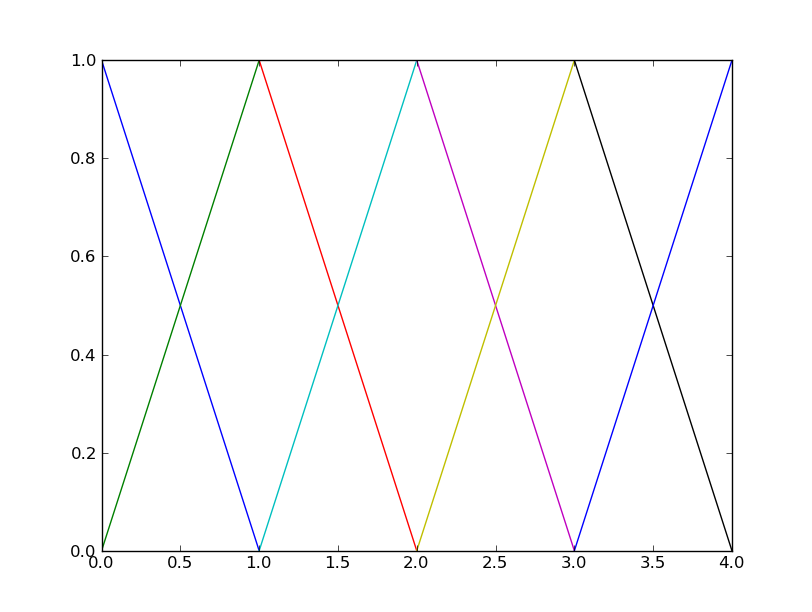
\includegraphics[width=225pt, height=150pt]{femexample1.png}
\caption[\textwidth]{FEM axis. n=4, order=1}
\end{figure}
The different elements are distinguished by colour.

The ``cosine eigenvectors'' are computed using \eqref{cosevec} and \eqref{freeschroedinger}.
The energies of the free wavefunctions are $E_n = n^2\pi^2/200$ for $n=0,\ldots,19$. The factor
of $200$ is a result of the discretization. The Green's operator, $G(z)$ is calculated for $z=E_n+i\epsilon$,
where, $\epsilon$ is a small positive number defined based on the problem. The purpose of epsilon is to avoid 
the singularity on the positive real axis.

\subsection{First Case}
In the first case, we define the potential as a finite well of strength $0.01$ with support in $4.5 \leq x \leq 5.5$,
\begin{equation}\label{potentialdef1}
V = \begin{cases}
-0.01 &\mbox{} 4.5\leq x\leq 5.5\\
0 &\mbox{ otherwise}
\end{cases} 
\end{equation}

\begin{center}
\begin{figure}[ht]
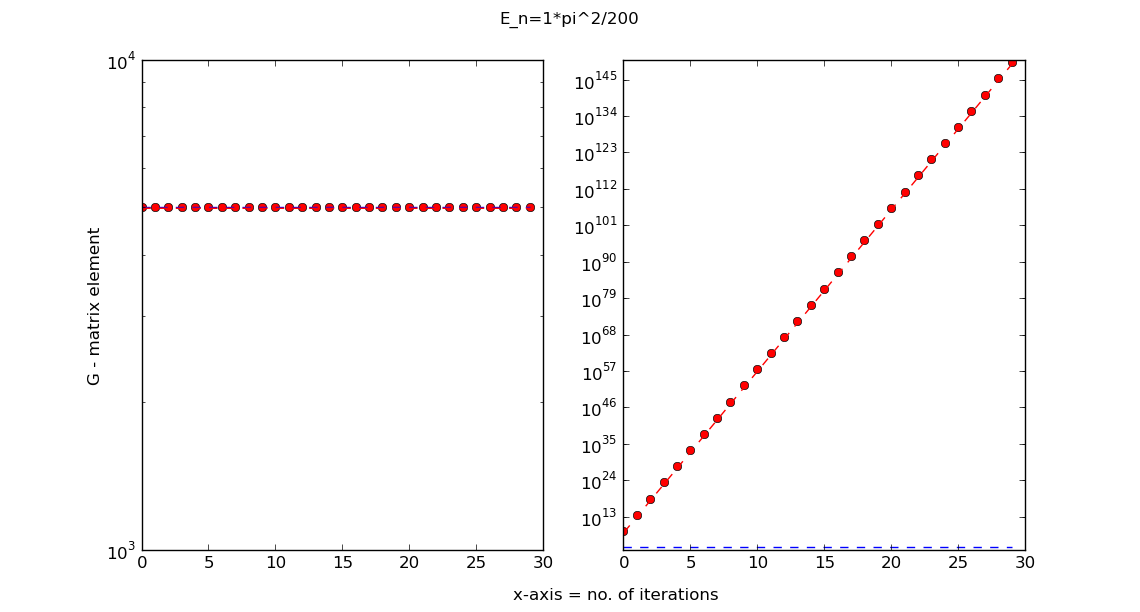
\includegraphics[width=360pt, height=175pt]{series1a.png}
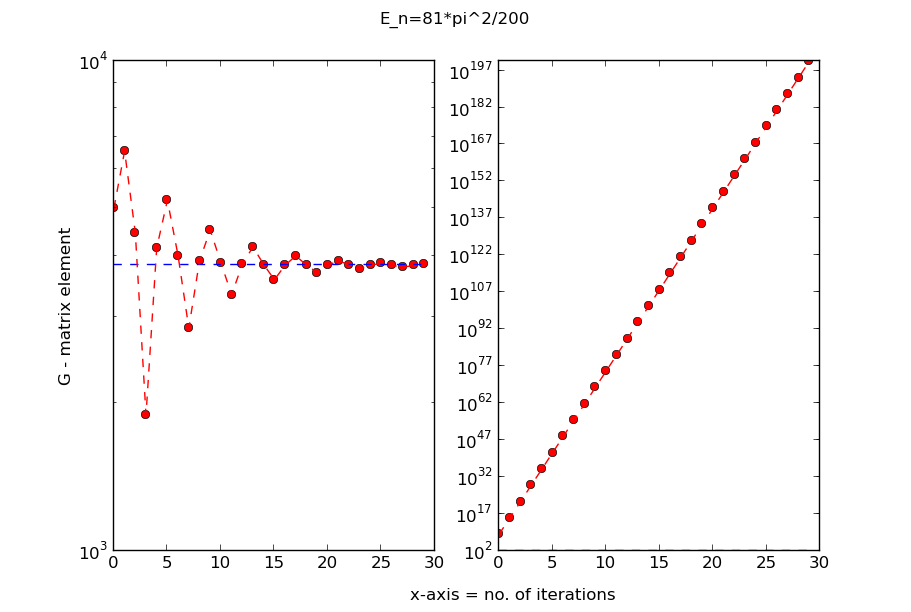
\includegraphics[width=360pt, height=175pt]{series1b.png}
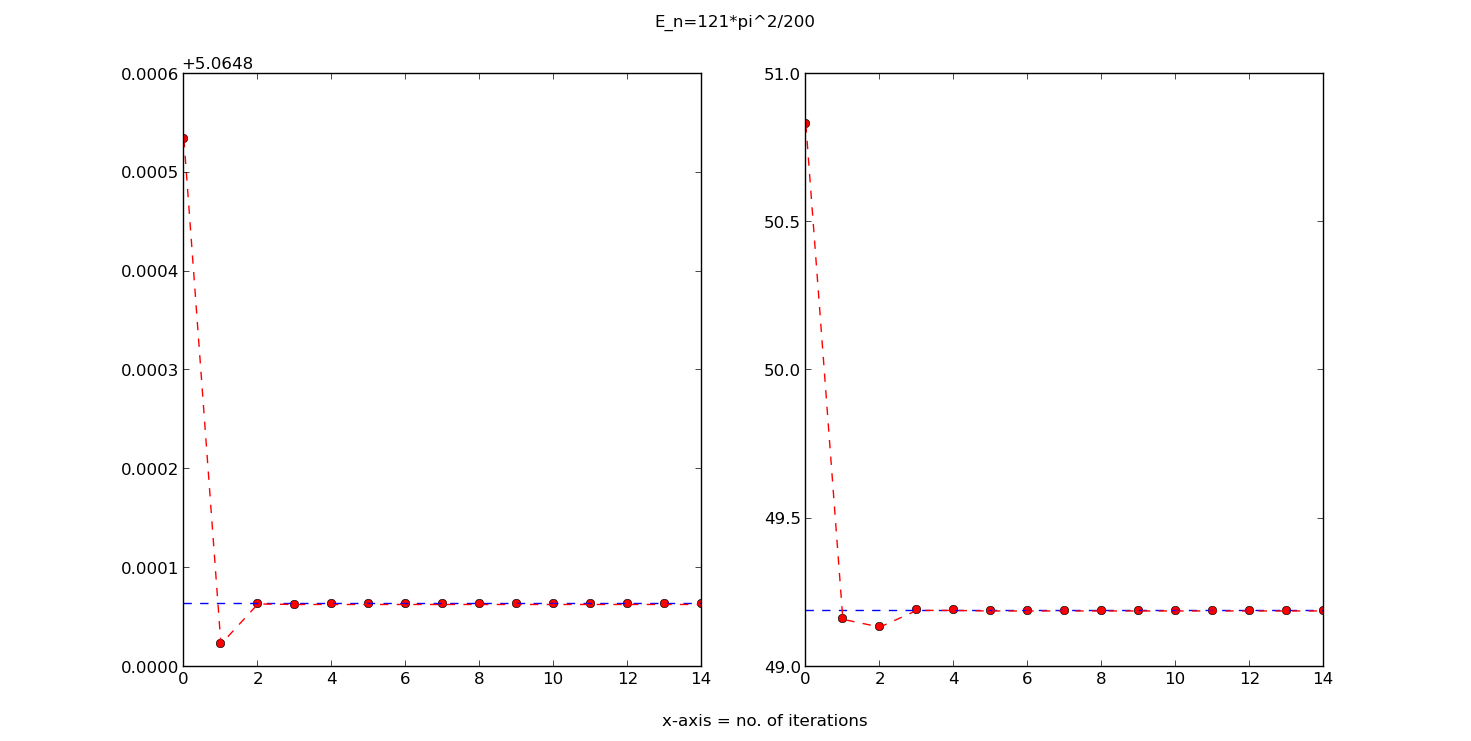
\includegraphics[width=360pt, height=175pt]{series1c.png}
\caption[\textwidth]{First Case - Weak Finite Well}
\end{figure}
\end{center}
The Born Series is calculated for $15$ iterations. The Hamiltonian is modified using the operator defined in \eqref{potmod} with
$\lambda=1$.  We also set $\epsilon=10^{-4}$. 

We now plot the elements of the Born Series against the number of iterations. In order
to compare the modified and unmodified cases, we plot them side by side with the modified case on the left and the unmodified one
on the right. We follow this convention in the other next case as well.
We see that the series converges in both cases.

\newpage
\subsection{Second Case}
\begin{equation}\label{potentialdef3}
V = -100\mathtt{exp}(-(x-3.5)^2/0.5)-100\mathtt{exp}(-(x-6.5)^2/0.5)
\end{equation}
\begin{figure}[hb]
\centering
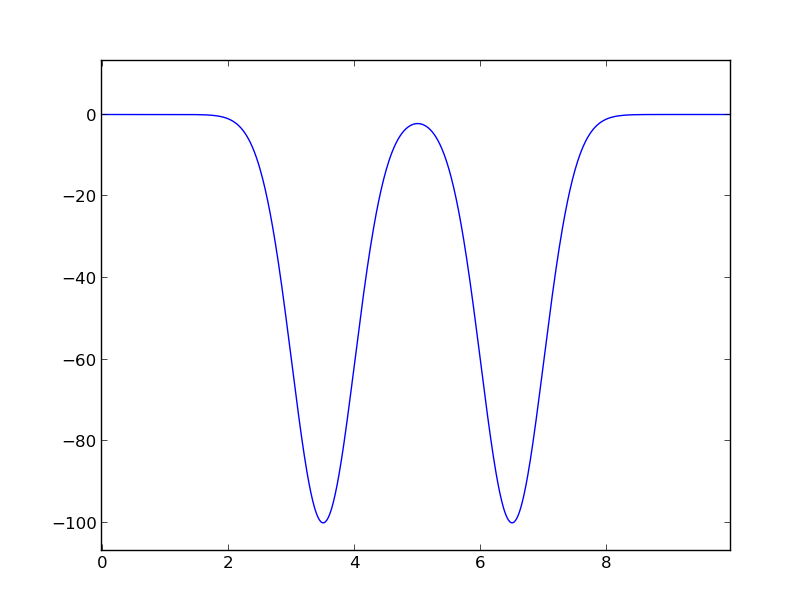
\includegraphics[width=225pt, height=150pt]{potential1d2.png}
\caption[\textwidth]{Test Potential 3}
\end{figure}

\begin{center}
\begin{figure}[lht]
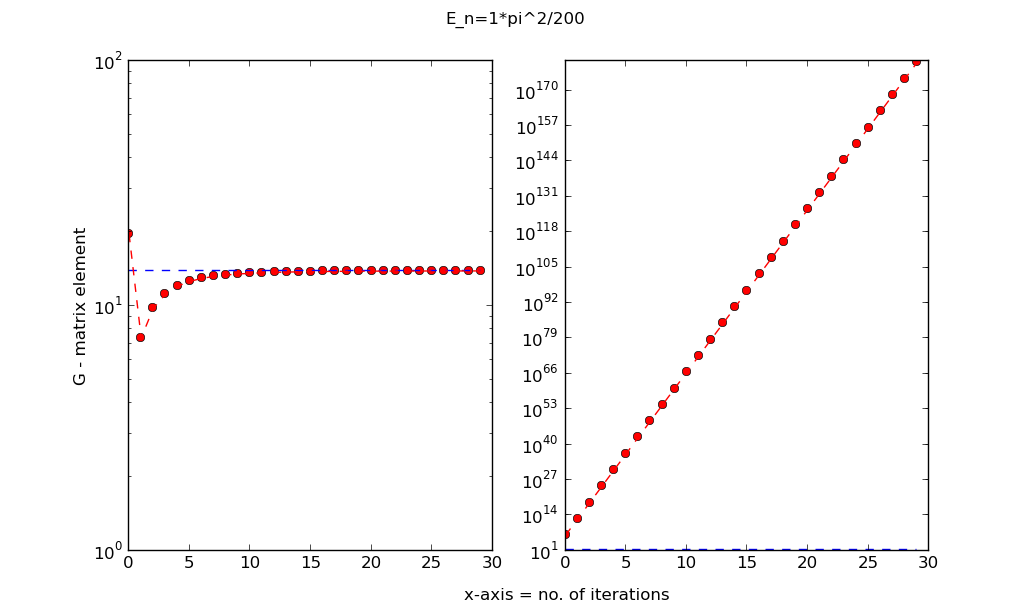
\includegraphics[width=360pt, height=200pt]{series3a.png}
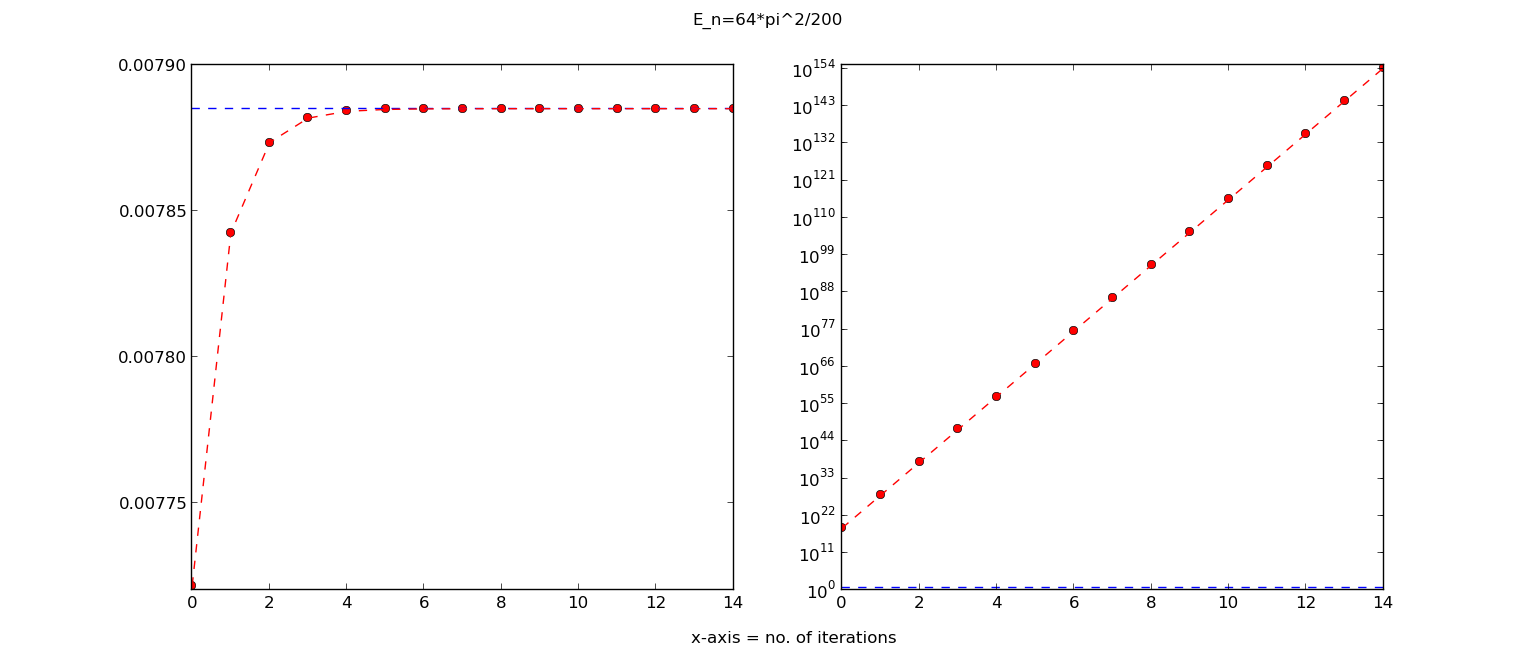
\includegraphics[width=360pt, height=200pt]{series3b.png}
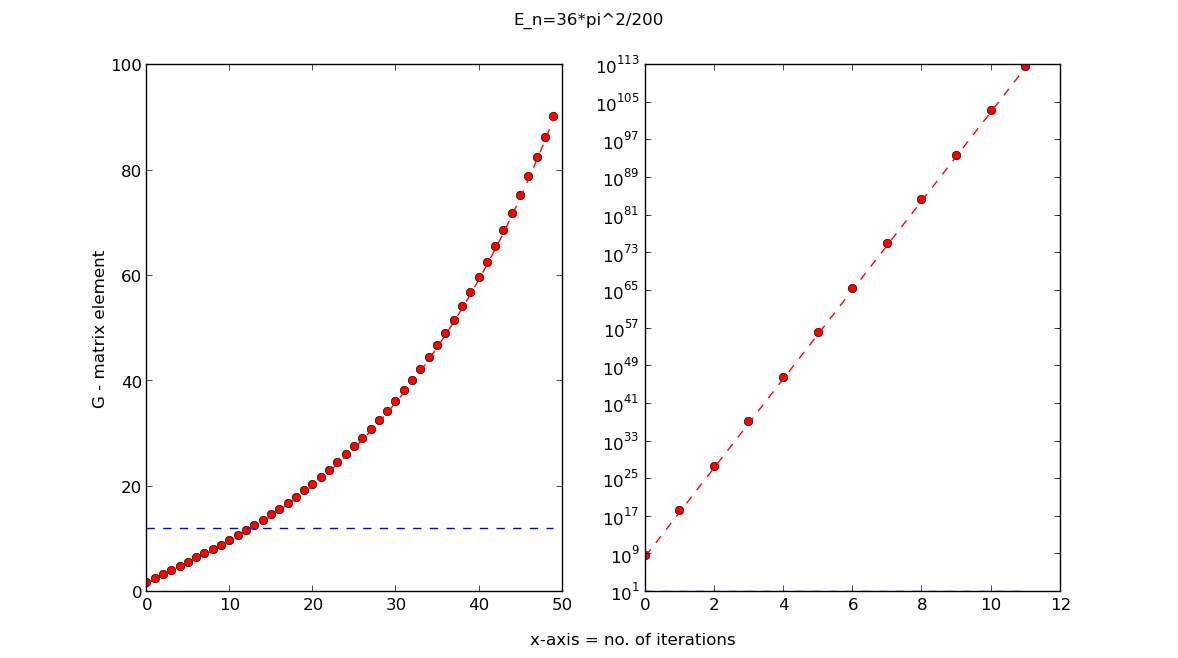
\includegraphics[width=360pt, height=200pt]{series3c.png}
\caption[\textwidth]{Gaussian Like Potential}
\end{figure}
\end{center}
% 
% \begin{center}
% \begin{figure}[lht]
% 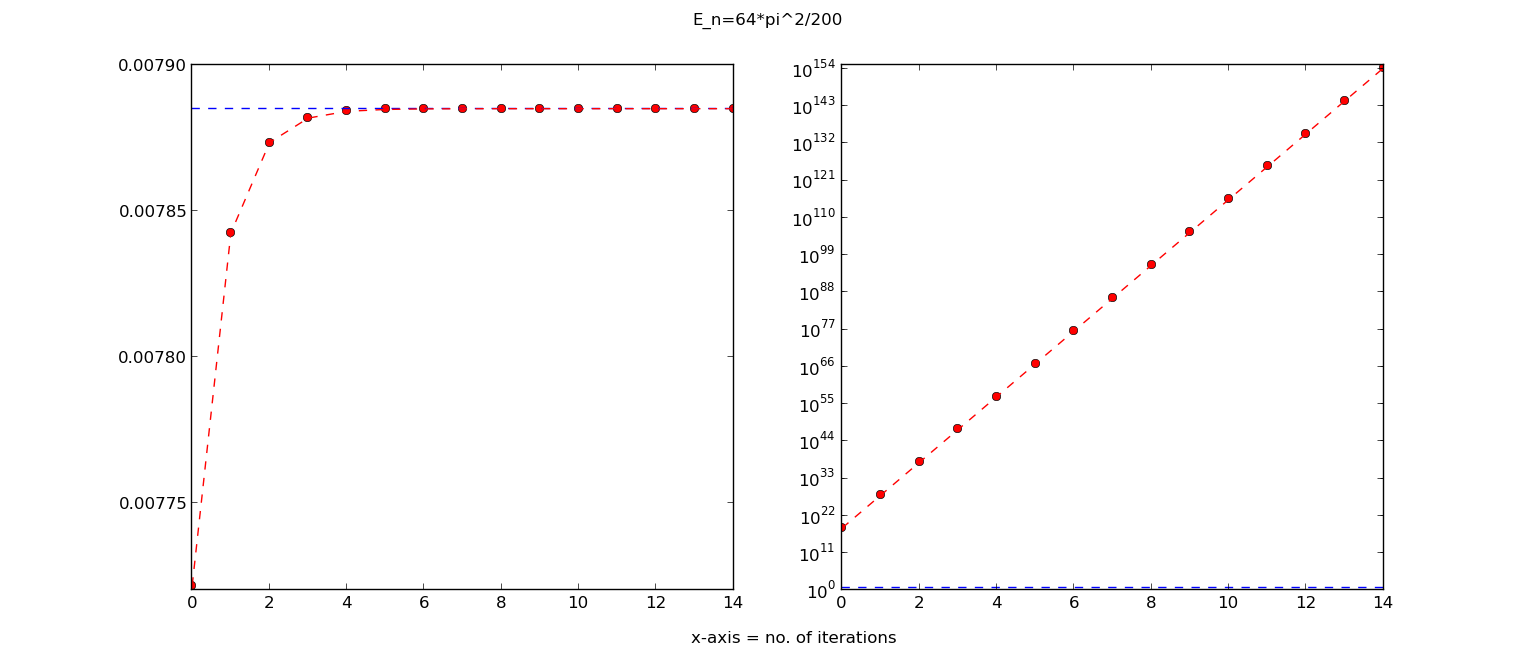
\includegraphics[width=360pt, height=200pt]{series3b.png}
% %\caption[\textwidth]{First Case}
% \end{figure}
% \end{center}
% 
% \begin{center}
% \begin{figure}[lht]
% 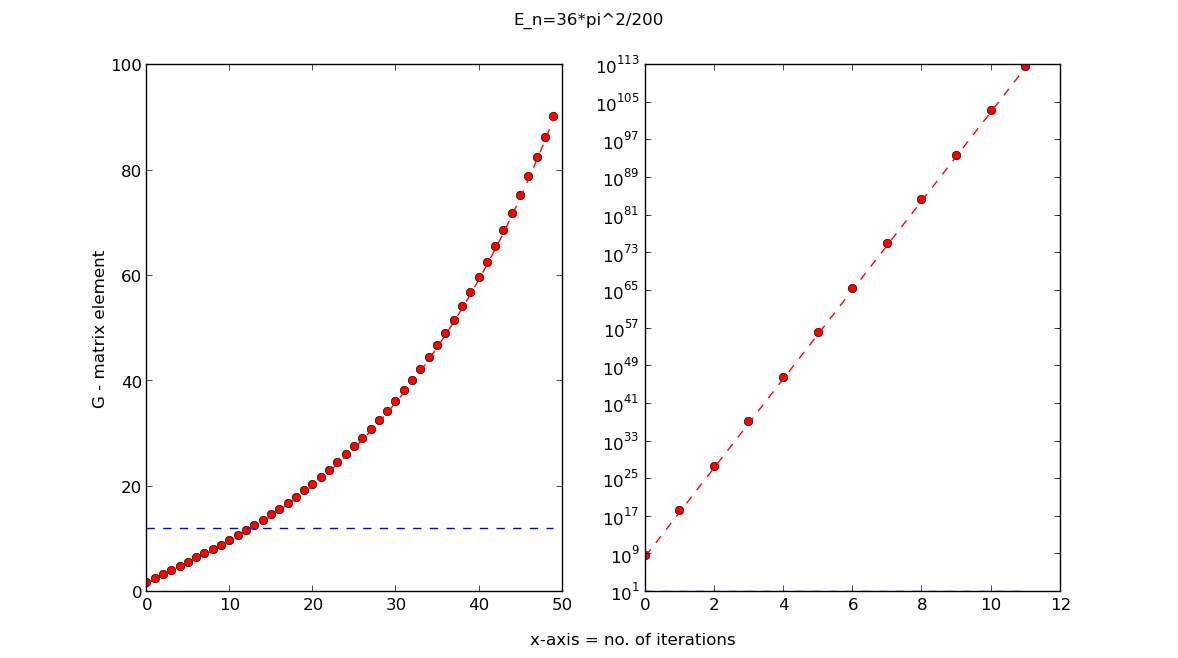
\includegraphics[width=360pt, height=200pt]{series3c.png}
% %\caption[\textwidth]{First Case}
% \end{figure}
% \end{center}

We see that for some energies the Born Series in the modified case converges to the exact value but diverges in the original case. We also note that
for certain energies, the Born Series diverges in both cases but the divergence in the unmodified case is slower.

\section{Conclusion}

\bibliographystyle{plain}
\bibliography{draft1.bib}
\end{document}
